\documentclass[UTF8]{ctexart}
\usepackage{geometry}
\geometry{margin=1.5cm, vmargin={0pt,1cm}}
\setlength{\topmargin}{-1cm}
\setlength{\paperheight}{29.7cm}
\setlength{\textheight}{25.3cm}

% useful packages.
\usepackage{amsfonts}
\usepackage{amsmath}
\usepackage{amssymb}
\usepackage{amsthm}
\usepackage{enumerate}
\usepackage{graphicx}
\usepackage{multicol}
\usepackage{fancyhdr}
\usepackage{layout}
\usepackage{listings}
\usepackage{xcolor}
\lstset{language=C++}
\setlength{\headheight}{13pt}  % 增加头部高度
\usepackage{float, caption}

% Listings setting for code formatting
\lstset{
    basicstyle=\ttfamily,
    keywordstyle=\color{blue},
    commentstyle=\color{gray},
    stringstyle=\color{red},
    breaklines=true,
    frame=single,
    numbers=left,
    numberstyle=\tiny,
    stepnumber=1,
    tabsize=4
}

% some common commands
\newcommand{\dif}{\mathrm{d}}
\newcommand{\avg}[1]{\left\langle #1 \right\rangle}
\newcommand{\difFrac}[2]{\frac{\dif #1}{\dif #2}}
\newcommand{\pdfFrac}[2]{\frac{\partial #1}{\partial #2}}
\newcommand{\OFL}{\mathrm{OFL}}
\newcommand{\UFL}{\mathrm{UFL}}
\newcommand{\fl}{\mathrm{fl}}
\newcommand{\op}{\odot}
\newcommand{\Eabs}{E_{\mathrm{abs}}}
\newcommand{\Erel}{E_{\mathrm{rel}}}

\begin{document}

\pagestyle{fancy}
\fancyhead{}
\lhead{陈梓锐, 22435036}
\chead{数值分析第二次作业}
\rhead{Oct.19th, 2024}

\section{测试程序的设计思路}
\begin{enumerate}
    \item 在 \texttt{Function.h} 里，定义了 \texttt{Function} 和 \texttt{Interpolation}类。
        其中Function类有两个虚函数,分别用于计算函数值和导数值。
        Interpolation是一个基类,用于插值,他有派生类Newtoninterpolation和Hermiteinterpolation,
        分别用于计算newton和hermite插值。
    \par 1.参数: Interpolation有参数points,用于存放插值点;laues用于存放函数在插值点处的值;
        n用于记录插值点的个数;x用于在得到的插值多项式计算函数值;differs用于存放差商表。
    \par 2.函数: Interpolation包括一个构造函数,一个求解函数solve和一个生成差商的函数generatediffs(这是一个纯虚函数),
        构造函数是默认构造函数,需要参数points,values和x;solve和generatediffs都是不需要参数的。
    \item \texttt{Hermiteinterpolation.h}里构造了定义了Hermiteinterpolation类,继承自Interpolation类。
    
        他只有两个函数:构造函数和差商生成函数generatediffers。
    \par 1.参数: Hermiteinterpolation比interpolation多了一个参数values\_用于存放函数在插值点处的值;
    \par 2.函数: Hermiteinterpolation构造函数需要参数points,values,values\_,n,x;
        函数generatediffers重写了父类中的差商生成函数。

    \item \texttt{Newtoninterpolation.h}里构造了定义了Newtoninterpolation类,继承自Interpolation类。
        他只有两个函数:构造函数和差商生成函数generatediffers。
    \par 1.参数: Newtoninterpolatione完全继承父类的参数,并不需要额外个参数；
    \par 2.函数: Newtoninterpolation构造函数需要参数points,values,n,x;
        函数generatediffers重写了父类中的差商生成函数。

    \item \texttt{Beziercurve.h}BezierCurve里定义了BezierCurve类,用于存储bezier曲线的控制点,控制点对应的函数导数值,以及存储每个分段bezier曲线的向量eachBezierCurves。
    子类eachBezierCurve用于对分段的bezier曲线进行处理。

    具体实现如下:
    \par 类 eachBezierCurve:
    \par 成员变量: 
    1. q: 用于存放四个控制点的值。
    2. a, b: 用于存放区间范围。
    \par 构造函数: 初始化区间 a 和 b, 计算贝塞尔曲线的控制点 q[0] 到 q[3]，基于函数值和导数值。
    \par 方法:
        1. solve(x): 计算参数 x 处的贝塞尔曲线值。
        2. combination(n, k): 计算组合数。
        3. bernstein(n, k, t): 计算 Bernstein 多项式。
        4. updateq(t): 更新 q 中存储的控制点的值。
        5. isInsegment(x): 检查 x 是否在当前区间范围内。
    \par 类 BezierCurve:
    \par 成员变量:
    1. points : 存放函数的离散点。
    2. values : 存放每个点的函数值。
    3. values\_: 存放每个点的导数值。
    4. eachBezierCurves: 存放每个区间的 eachBezierCurve 对象。
    \par 构造函数: 接收离散点、函数值、导数值并进行初始化。
    \par 方法:
        1. segment(): 对所有区间进行分段，并为每段生成对应的 eachBezierCurve 对象。
        2. solveP(x): 计算给定 x 值的贝塞尔曲线值，遍历所有区间，找到对应的 eachBezierCurve，并调用其 solve(x)。


    \item \texttt{ProblemB.cpp}是第B题的程序,首先定义了函数f即题目要求的rough函数,
        在编译后,运行可执行文件,会需要输入相应的n值。这时程序会自动构造好插值节点points,生成插值多项式,
        在给定区间上的x不断使用插值多项式计算函数值,将结果写入文件“outputB.dat”,我们只需要在终端输入
        gnuplot,plot outputB.dat,即可获得函数图像。

        \par n = 2, \par 
\includegraphics[width=0.75\textwidth]{pic/B2.png}
        \par n = 4, \par 
\includegraphics[width=0.75\textwidth]{pic/B4.png}
        \par n = 6, \par 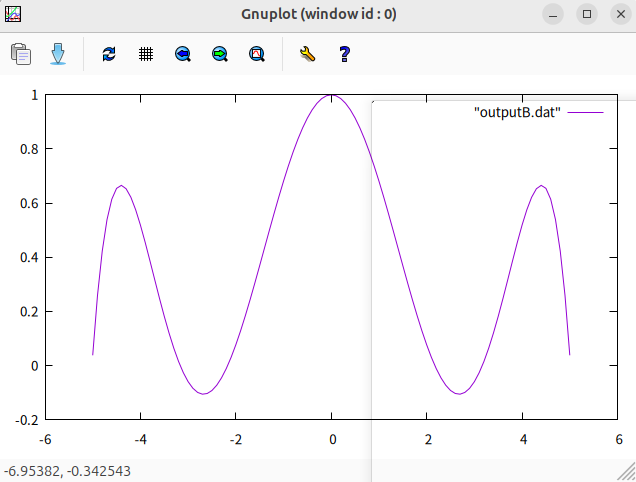
\includegraphics[width=0.75\textwidth]{pic/B6.png}
        \par n = 8, \par 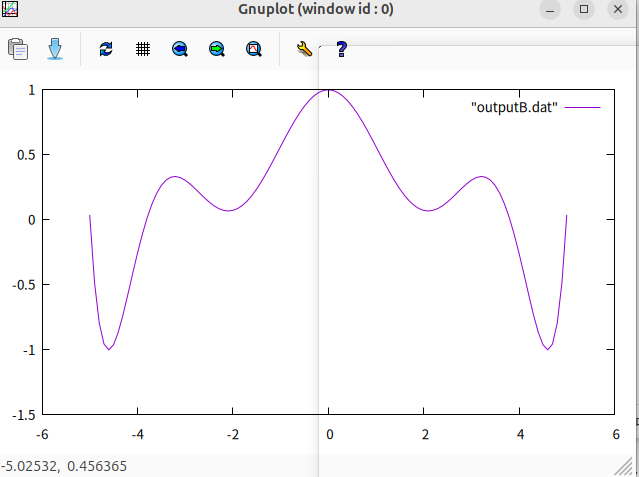
\includegraphics[width=0.75\textwidth]{pic/B8.png}

    \item \texttt{ProblemC.cpp}是第C题的程序,本质上跟第B题是一样的,区别在于插值点变为
        chebyshev多项式的根。 
        \par n = 5, \par 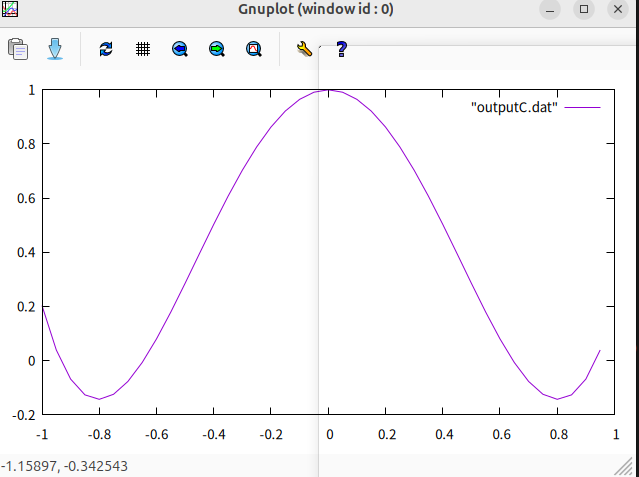
\includegraphics[width=0.75\textwidth]{pic/C5.png}
        \par n = 10, \par 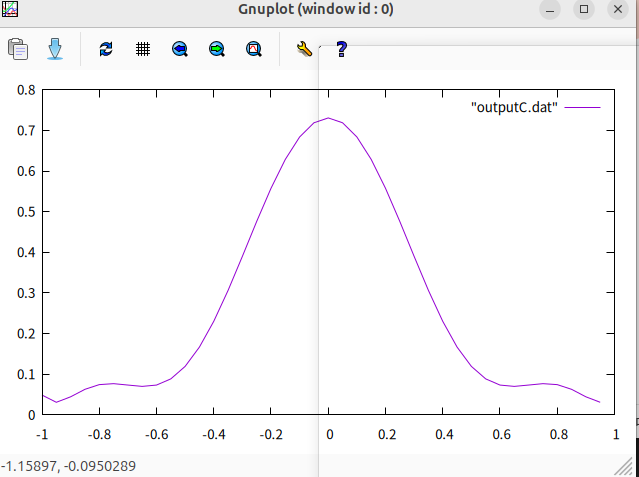
\includegraphics[width=0.75\textwidth]{pic/C10.png}
        \par n = 15, \par 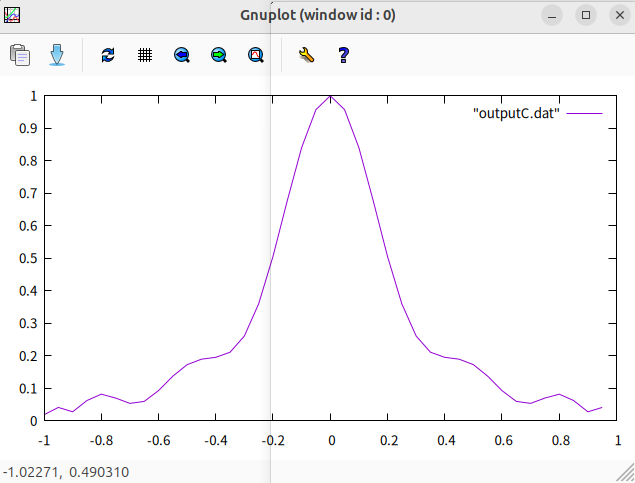
\includegraphics[width=0.75\textwidth]{pic/C15.png}
        \par n = 20, \par 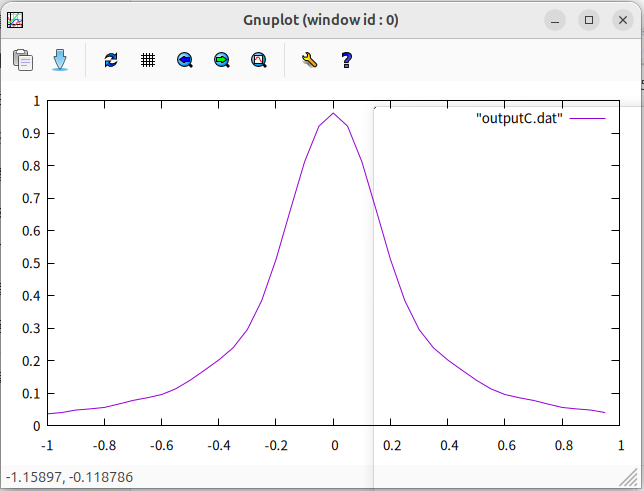
\includegraphics[width=0.75\textwidth]{pic/C20.png}

    \item \texttt{ProblemD.cpp}是第D题的程序,计算Hermite多项式的插值,在a问中我们通过计算导数算出
        小车在t等于10的速度估计。

        \par t = 10, \par 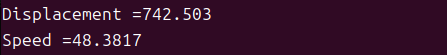
\includegraphics[width=0.75\textwidth]{pic/D.png}

        \par 第二问b不会。


    \item \texttt{ProblemE.cpp}用newton插值画图。
        \par sp1 \par 
\includegraphics[width=0.75\textwidth,height = 8cm]{pic/E1.png}
        \par sp2 \par 
\includegraphics[width=0.75\textwidth]{pic/E2.png}
        \par 第二问不知道如何判断是否存活,以下是在43处的输出。
        \par 
\includegraphics[width=0.75\textwidth]{pic/E3.png}


    \item \texttt{ProblemF.cpp}
        我们只需要在ProblemF.cpp里调用BezierCurve类,并传入控制点,和我们想要的x值,就可以得到bezier曲线在x处的值。运行可执行文件F后, 在终端输入gnuplot, 
        \par set xrange[-2:2]
        \par set yrange[-2:2]
        \par plot 'outputF1.dat' using 1:2 with lines title 'Output F1', \
        \par'outputF2.dat' using 1:2 with lines title 'Output F2' 即可获得如下图像。

        \par m = 10 :\par 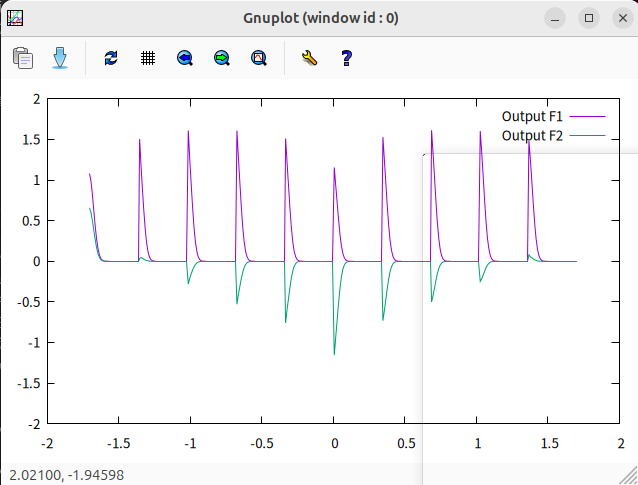
\includegraphics[width=0.75\textwidth]{pic/F10.png}
        \par m = 40 :\par 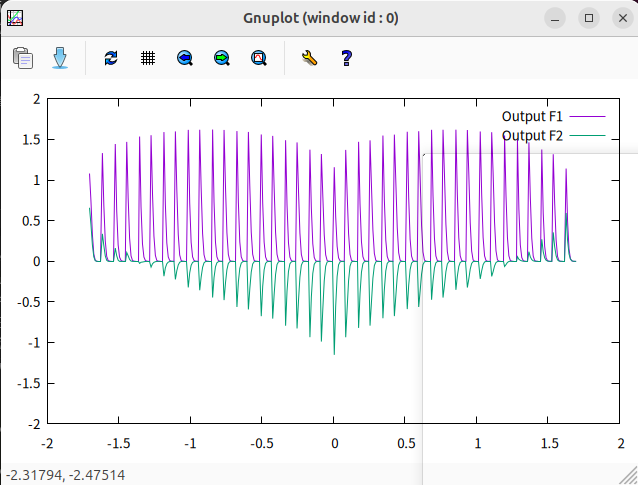
\includegraphics[width=0.75\textwidth]{pic/F40.png}
        \par m = 160 :\par 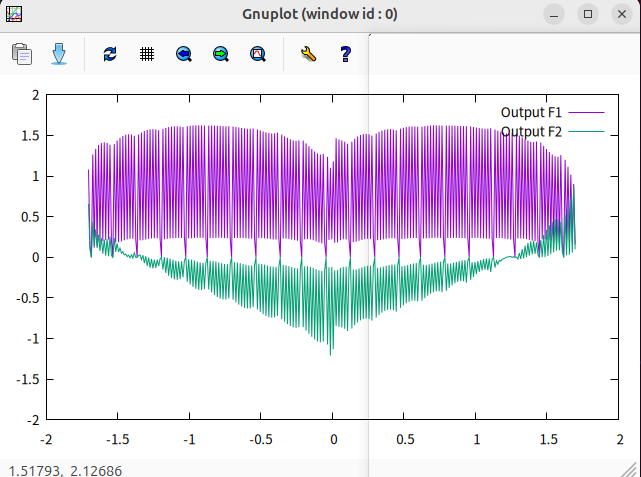
\includegraphics[width=0.75\textwidth]{pic/F160.png}
\end{enumerate}

\section{部分代码}
\subsection{solver}
\begin{lstlisting}[language=C++]
double Interpolation::solve() {
    generatediffers();
    double fx = 0.0;
    double h;
    double x = this->x;
    for(int i = n; i >= 2; --i) {
        h = x - points[i - 2];
        fx = h * (fx + differs[i - 1][i - 1]);
    }
    fx += differs[0][0];
    return fx;
}
    

\end{lstlisting}

\subsection{Newton's generatediffers}
\begin{lstlisting}[language=C++]
void NewtonInterpolation::generatediffers() {
    differs.resize(n, std::vector<double>(n, 0.0));
    for(int i = 0; i < n; i++){
        differs[i][0] = values[i];
    }
    for(int j = 1;j < n;j++){
        for( int i = j; i < n; i++){
            differs[i][j] = (differs[i][j-1] - differs[i-1][j-1])
                            /(points[i]-points[i-j]);
        }
    }
}
\end{lstlisting}

\subsection{Hermite's generatediffs}
\begin{lstlisting}[language=C++]
differs.resize(n, std::vector<double>(n, 0.0));
for(int i = 0 ;i < n;i++){
    differs[i][0] = values[i] ;
}
int s = 0;
for(int i = 1;i < n;i++){
    if(points[i] != points[i-1]){
            differs[i][1] = (differs[i][0] - differs[i-1][0])
                                /(points[i]-points[i-1]);
    }
    else{
        differs[i][1] = values_[s]; 
        ++s;
    }
}
for(int j = 2;j < n;j++){
    for( int i = j; i < n; i++){
        differs[i][j] = (differs[i][j-1] - differs[i-1][j-1])
                        /(points[i]-points[i-j]);
    }
}
\end{lstlisting}

\subsection{Bezier curve}
\begin{lstlisting}[basicstyle=\ttfamily]
    class eachBezierCurve:
    - q: list of control points
    - a, b: range of the segment

    eachBezierCurve(points, values, derivatives):
        initialize a and b with points
        calculate control points q based on values and derivatives

    solve(x):
        calculate normalized t based on x in the range [a, b]
        update control points q based on Bernstein polynomials
        return the evaluated Bezier curve value at x

    combination(n, k):
        return combination number C(n, k)

    bernstein(n, k, t):
        return the value of the Bernstein polynomial B(n, k, t)

    updateq(t):
        update q using Bernstein polynomials for t

    isInsegment(x):
        return true if x is in the range [a, b]


class BezierCurve:
    - points, values, derivatives: lists of points, function values, and derivatives
    - eachBezierCurves: list of eachBezierCurve objects

    BezierCurve(points, values, derivatives):
        initialize with points, values, and derivatives

    segment():
        for each segment between points:
            create an eachBezierCurve and store it

    solveP(x):
        for each segment in eachBezierCurves:
            if x is in the segment:
                return the Bezier curve value at x

main(ProblemF):
    define function F(x) and its derivative
    initialize start and end points, number of segments m
    compute points, values, and derivatives for the function
    create BezierCurve object
    segment the curve
    for each x in the range [xStart, xEnd]:
        compute Bezier curve value using solveP(x)
        write the result to a file


\end{lstlisting}



\end{document}
